% Redrawn figure 79/14-1 of the edition (transcripts/79/drawings/14-1.tex), copied for this article.
% Drawing 79/14-1 -- folder 79, batch 14, archive page 275 (PDF page 276).
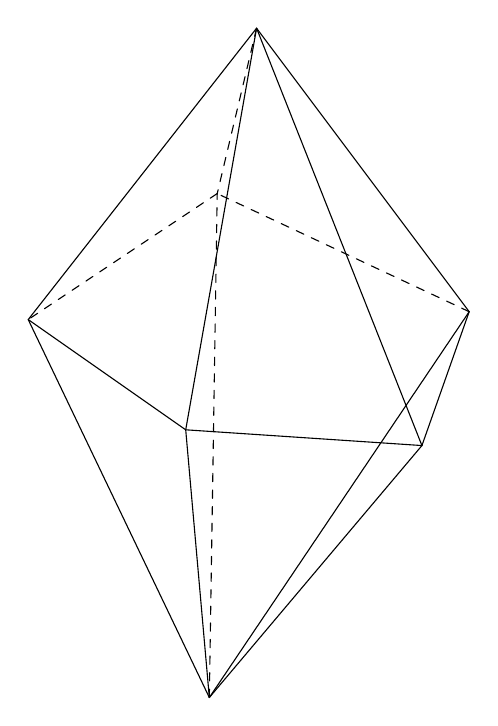
\begin{tikzpicture}[pencil/.style={black!45}, struck/.style={black!35}, mark/.style={circle,draw,inner sep=1.3pt}, pt/.style={circle,fill,inner sep=0.9pt}, opt/.style={circle,draw,fill=white,inner sep=1.1pt},x=1mm,y=1mm,line cap=round,line join=round,font=\scriptsize]
\draw (10,-58) -- (30,-72);
\draw (30,-72) -- (60,-74);
\draw (60,-74) -- (66,-57);
\draw (39,-21) -- (10,-58);
\draw (39,-21) -- (30,-72);
\draw (39,-21) -- (60,-74);
\draw (39,-21) -- (66,-57);
\draw (33,-106) -- (10,-58);
\draw (33,-106) -- (30,-72);
\draw (33,-106) -- (60,-74);
\draw (33,-106) -- (66,-57);
\draw[dashed] (66,-57) -- (34,-42);
\draw[dashed] (34,-42) -- (10,-58);
\draw[dashed] (39,-21) -- (34,-42);
\draw[dashed] (33,-106) -- (34,-42);
\end{tikzpicture}
